\chapter{Edición vectorial y estadísticas}\label{ap:EV}

Para calcular estadística sobre vectores deben realizarse dos pasos.

\section{Creación de vectores}

Cree un contenedor vectorial haciendo click en \menu{Vector>New Vector Data Container}. Nombrelo \path{Urbano} (Figura \ref{fig:vector-cont}). Seleccione luego la herramienta \menu{Rectangle drawing tool} de la barra de herramienta y digitalice un rectángulo sobre la zona urbana. Para confirmar la geometría haga click fuera de ella.

\begin{figure}[h!]
    \centering
    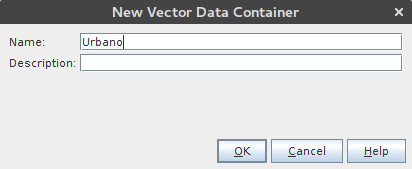
\includegraphics[scale=0.4]{fig:vector-cont.png}
    \caption{Herramenta de creación de contenedores vectoriales. Debe serse un nombre único a cada uno y puede agregarse una descripción.}
    \label{fig:vector-cont}
\end{figure}

Puede crear varias geometrías dentro de un mismo vector o crear distintos contenedaros vectoriales. Estos quedarán asociados al archivo haciendo y se guardarán haciendo click derecho sobre el nombre de la imagen y seleccionando \menu{Save product}.

\section{Estadística}

Haga click en \menu{Analysis>Statistics}. Una vez abierta la ventana tilde la opción \texttt{Use ROI maks(s)} (Figura \ref{fig:estadistica}).

\begin{figure}[ht!]
    \centering
    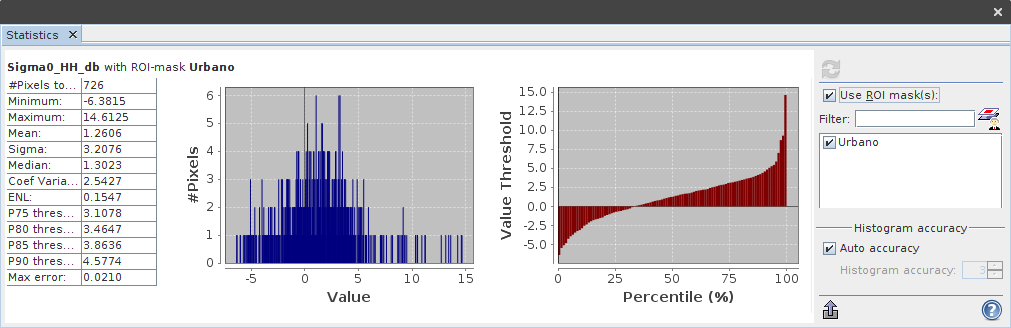
\includegraphics[scale=0.35]{fig:estadistica.png}
    \caption{Calculo de parámetros estadísticos en SNAP. Es posible calcularlos sobre una región seleccionando \menu{Use ROI maks(s)} y luego la región de interés.}
    \label{fig:estadistica}
\end{figure}

 Seleccione la región Urbano, haga click en el botón \menu{Refresh view}. El SNAP calculará la estadística sobre el vector. Puede hacerlo para varias regiones en simultaneo.
